 % this file is prim_tools.tex
 
  
  \section{Pollard Rho Methode}
  \label{sec:pollard}
  \subsection{Geburtstagsproblem}
  Die Idee des Geburtstagsproblems ist die Frage, wie hoch die Wahrscheinlichkeit auf einem Geburtstag mit $N$ Personen ist, dass zwei Personen am gleichen Tag Geburtstag haben.\\
  Eine M\"oglichkeit das Problem einfacher zu machen ist, stattdessen das inverse Problem zu betrachten, also wie hoch die Wahrscheinlichkeit $(P)$ ist, dass kein Geburtstag doppelt vorkommt.\\
  Bei einem Besucher ist die Wahrscheinlichkeit
  \[P(1)=\frac{356}{356}\] 
  da alle $356$ Tage zur Wahl stehen. Bei zwei Besuchern ist die Wahrscheinlichkeit 
  \[P(2)=\frac{356}{356}\cdot \frac{364}{365}\]
  bei drei Besuchern gilt  
  \[P(3)=\frac{356}{356}\cdot \frac{364}{365} \cdot \frac{363}{365}\]
  Im Allgemeinen gilt: 
  \[P(N)= \frac{365 \cdot 364 ... (365-N+1)}{365^N}\]
  Da wir gro\ss e Primzahlen betrachten werden interessiert uns auch das Verhalten des Geburtstagsproblems f\"ur gro\ss e $N$.
  Beim Betrachten von vielen Geburtstagen mit $N$ Personen liegt, f\"ur gro\ss e N, die Zahl der Wiederholungen die man durchschnittlich braucht um einen doppelten Geburtstag zu erhalten bei: 
  \[\sqrt{\frac{\pi \cdot N}{2}}\]
  
  \subsection{Hase Igel Algorithmus}
  \label{sec:hase}
  Der Hase Igel Algorithmus wird benutzt, um Zyklen in Folgen zu finden. Die Idee ist, die Folge mit zwei Zeigern zu durchlaufen, dem Hase und dem Igel, die auf dem gleichen Feld starten. Falls es einen Zyklus in der Folge gibt, werden sich Hase und Igel irgendwann wieder treffen, da der schnellere Hase den langsameren Igel einholt und \"uberrundet.

  \subsubsection{Beispiel}
  In diesem Beispiel ist eine Folge zu sehen, die einen Zyklus beinhaltet. 
    %\newpage
    \begin{figure}[!h] 
    	\centering
    	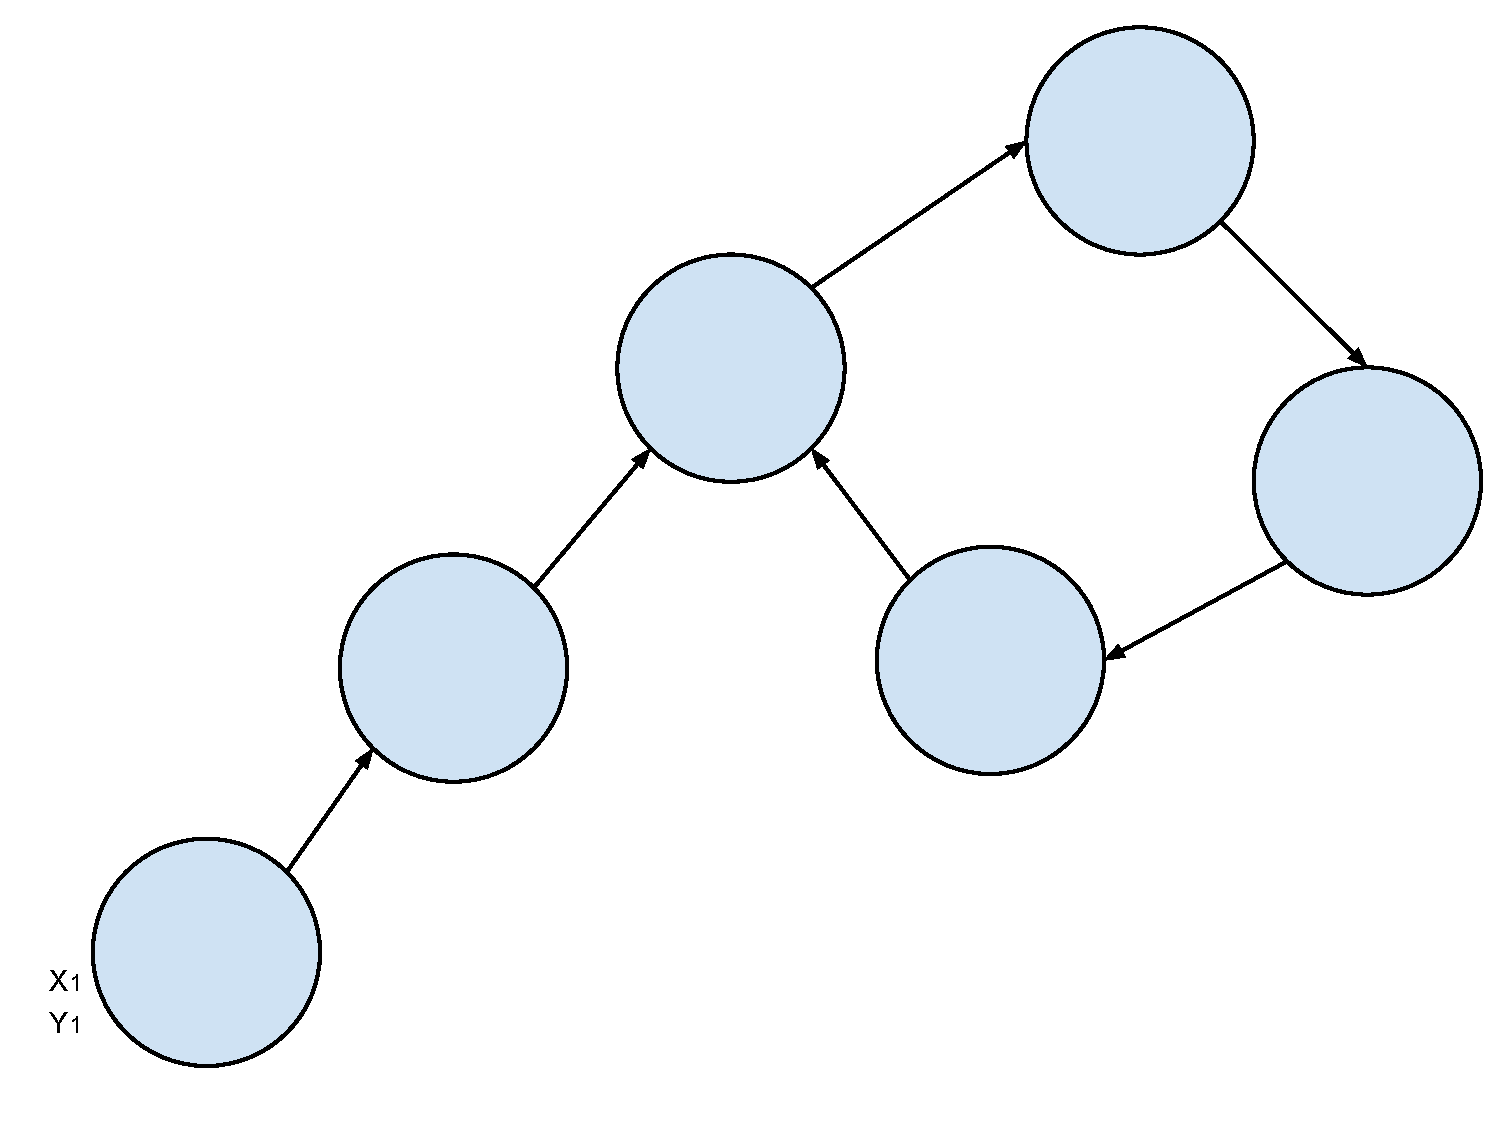
\includegraphics[width=0.7\linewidth]{Rho1}
    	\caption{Schritt 1}
    	\label{fig:Rho1)}
    \end{figure}
    
    \noindent Der Hase, hier dargestellt durch Y und der Igel, hier dargestellt durch X starten an der gleichen Position. Der Igel bewegt sich um ein Element, der Hase um zwei Elemente vorw\"arts.

  \begin{figure}[!h] 
  	\centering
  	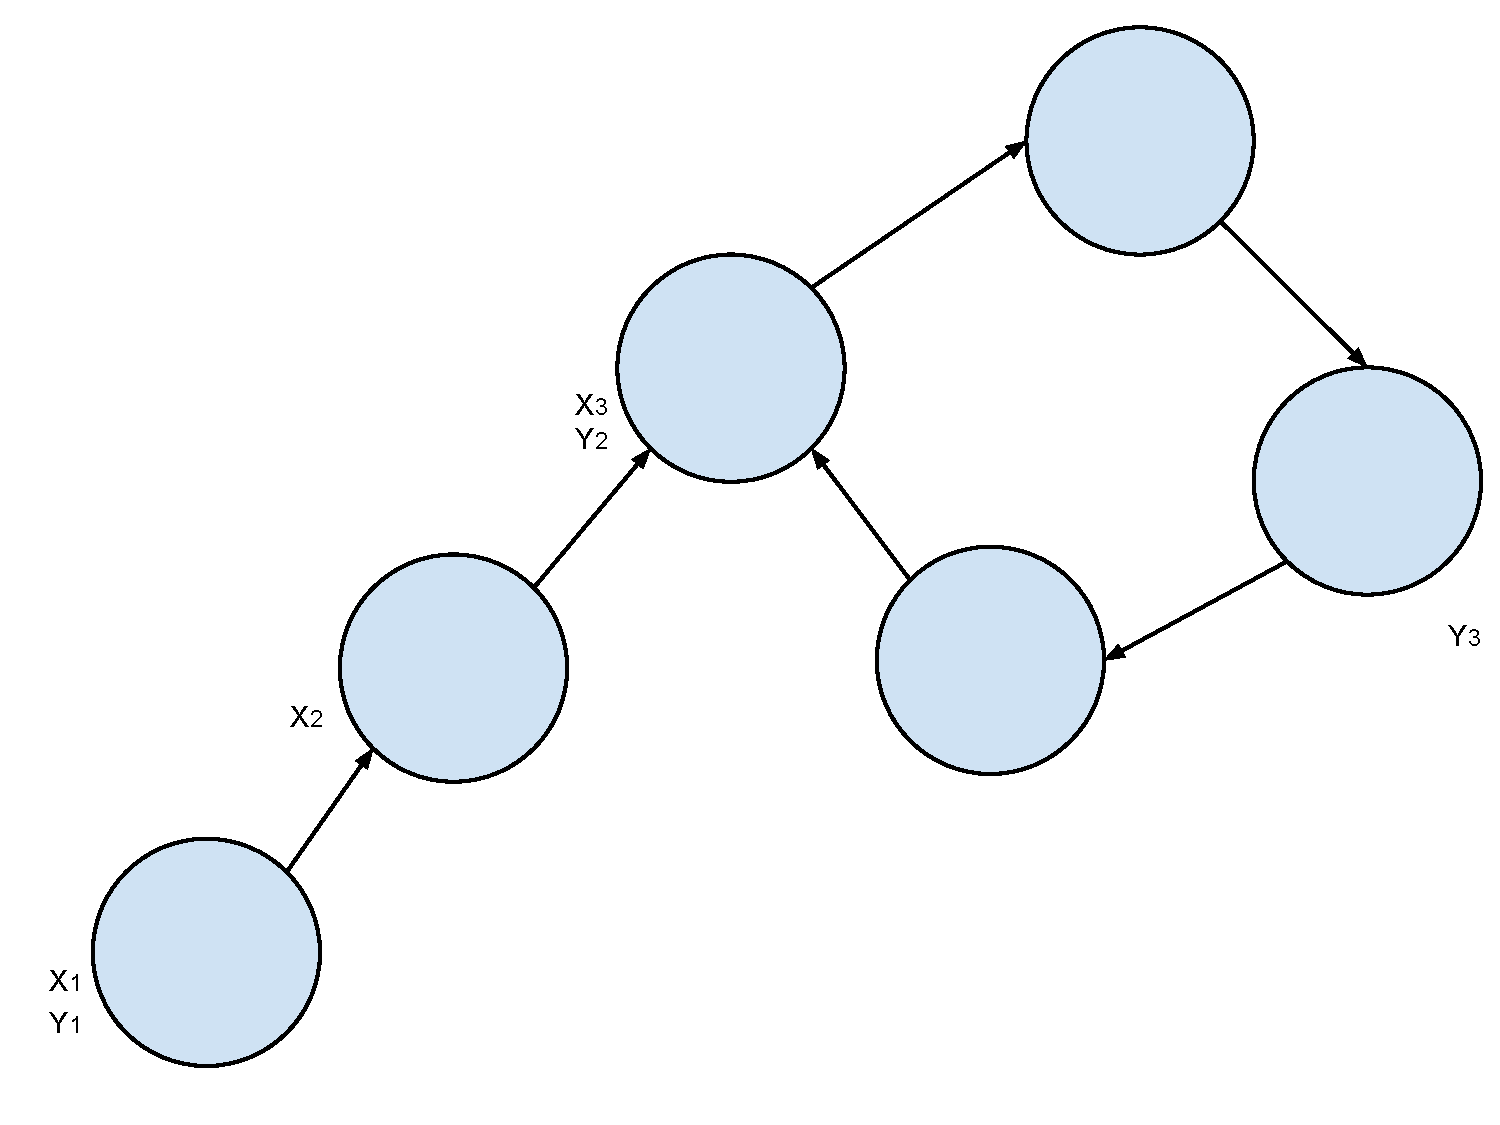
\includegraphics[width=0.7\linewidth]{Rho2}
  	\caption{Schritt 2}
  	\label{fig:Rho2)}
  \end{figure}
  
  \noindent Das ist der Zustand, bevor der Hase das erste mal im Kreis l\"auft. Es ist zu erkennen, dass der Hase doppelt so weit ist, wie der Igel.\\
  
    \begin{figure}[!h] 
    	\centering
    	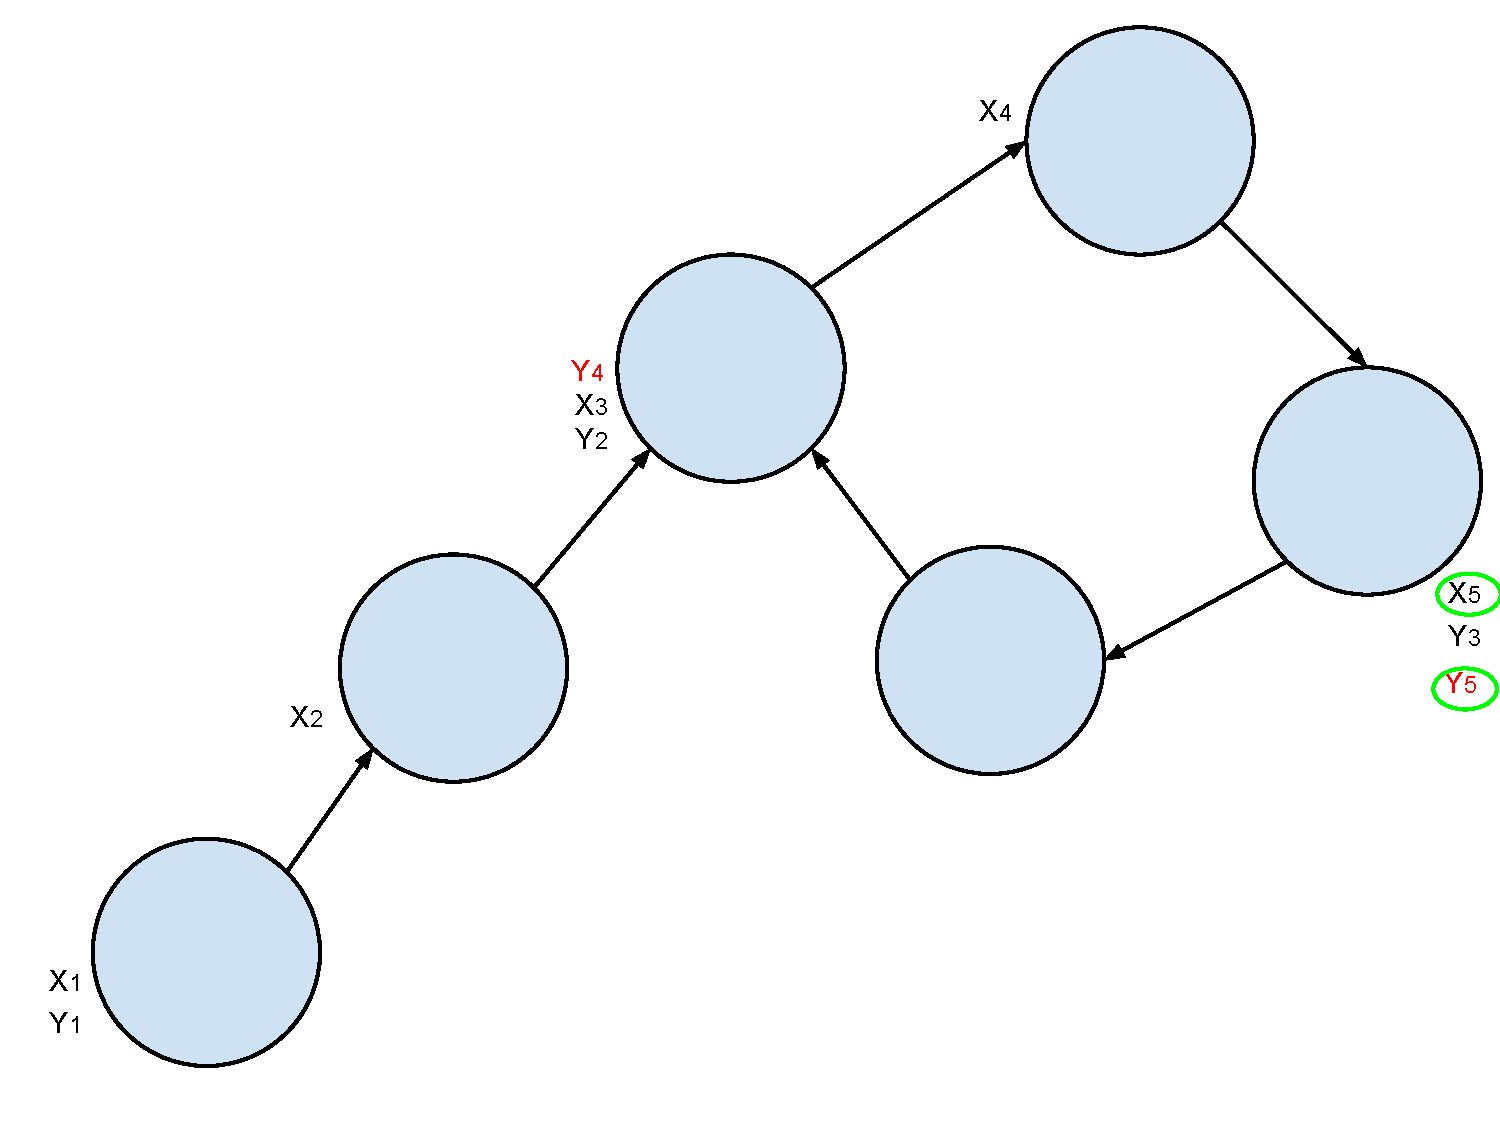
\includegraphics[width=0.7\linewidth]{Rho3}
    	\caption{Schritt 3}
    	\label{fig:Rho3)}
    \end{figure}
    \ \\
    Dies ist der Zustand, wenn Hase und Igel sich treffen. Die roten Zahlen zeigen, dass der Hase im Kreis l\"auft und die gr\"un eingekreisten Zahlen zeigen, dass Hase und Igel sich in ihrem f\"unften Schritt treffen. 

  \subsubsection{Mathematik}
  \begin{itemize}


  	\item Sei $M$ eine endliche Menge mit der Abbildung $f : M \rightarrow M$. Die Menge $M$ wird im Beispiel durch die Kreise dargestellt, die Abbildung $f$ durch die Pfeile, die die Kreise verbinden.
  	
  	\item Man w\"ahle $x_0 \in M$ und erzeuge die Folge $x_0, x_1, x_2,...$ mit $x_{i+1} = f(x_i)$. Dies wird im Beispiel durch den Igel dargestellt, der sich entlang der Pfeile mit einer Schrittweite von $1$ durch die Menge bewegt.
	
  	\item $\exists \ i,j \in \mathbb{N}$, sodass $i \not= j$ und $x_i = x_j$ gilt. Hiermit wird gesagt, dass es einen Zyklus gibt. Wenn der Igel zwei mal auf das gleiche Feld kommt, muss er im Kreis gegangen sein.
  	
  	\item Die Folge $y_0, y_1, y_2,...$ gegeben durch $y_0=x_0$ und $y_{i+1}=f(f(y_i))$ ist gleich der Folge $x_0,x_2,x_4,...$.\\
  Hiermit wird der Hase beschrieben, der sich doppelt so schnell bewegt wie der Igel. 
  	
  	\item Es gibt ein $c>0$, sodass $x_c=x_{2c}$.
  	 \end{itemize}
  	\noindent Dies ist die Bedingung daf\"ur, dass es m\"oglich ist, dass sich Hase und Igel wieder treffen und zwar wenn beide gleich viele Schritte gemacht haben. $c$ f\"ur den Igel, $2c$ f\"ur den Hasen, da der Hase eine doppelt so gro\ss e Schrittweite hat wie der Igel.
 
  
  Ein Beweis f\"ur diesen Algorithmus wird in Abschnitt \ref{sec:pollardBeweis} gef\"uhrt.